\section{Software Teori}
\textit{I dette afsnit beskrives den udleverede microcontroller, CY8CKIT-043 PSoC 4 M, og dens egenskaber. Dette gøres med henblik på at få forståelse for dens muligheder, og hvordan disse kan benyttes til udvikling af systemet.}

\subsection{Mikrokontroller}
En mikrokontroller er et elektrisk system, som kan kontrollere elektronisk udstyr ved hjælp af indlejret softwaredesign. En mikrokontroller kan derfor anses som en mindre computer, der findes indeni elektroniske enheder. Eksempelvis er mikrokontrollere at finde i fjernsyn, mobiltelefoner og printere. \citep{Scienceuddannelse,Tanenbaum2006} \newline
Mikrokontrollere kan være bestående af en eller flere mikroprocessorer, hukommelse samt programmerbare in- og output-enheder. Dette giver brugeren af mikrokontrolleren mulighed for at programmere enheden således, at denne kan kontrollere henholdsvis in- eller output-enheder. \citep{Scienceuddannelse,Tanenbaum2006}

\subsection{CY8CKIT-043 PSoC 4-M og PSOC Creater}
Til dette projekt anvendes mikrokontrolleren CY8CKIT-043 Programmable System on Chip (PSoC) 4 M-Series Prototyping Kit og programmet PSoC Creater til at opsamle det biologiske signal.\\
CY8CKIT-043 PSoC 4 M-Series Prototyping Kit er en prototyping platform, der indeholder tre mikroprocessorer: to Programmable System-on-Chips (PSoC) og en Programmable Radio on Chip (PRoC), hvilket ses på \figref{fig:PSoC}. Den første PSoC LP5 på mikrokontrolleren (MCU) sidder på KitProg boardet og kan indeholde programmer, der kan indlæses på en computer ved hjælp af USB stikket. Den bruges til at programmere og debug softwaren på target boardet af MCUen, hvorfor denne del kan knækkes af resten af stikket og fungere selvstændigt. Dette kræver dog, at softwaren først er programmeret på den anden mikroprocessorer, som er PSoC 4200M. Denne fungerer som hovedcomputeren, der programmeres på igennem c koden, og muliggøre eksempelvis høj-performans analog til digital konvertering igennem sin 12-bits SAR ADC. På bagsiden af MCUen sidder en PRoC med Bluetooth Low Energy (BLE). Denne PRoC har ikke lige så mange muligheder for afbenyttelse i forhold til PRoC 4200M, da BLE optager meget plads, hvorfor der ikke er plads til meget andet. \citep{CYPRESS2016PSoC,Semiconductor2016,CYPRESS2016Cortexm0}
\begin{figure}[H]
	\centering
	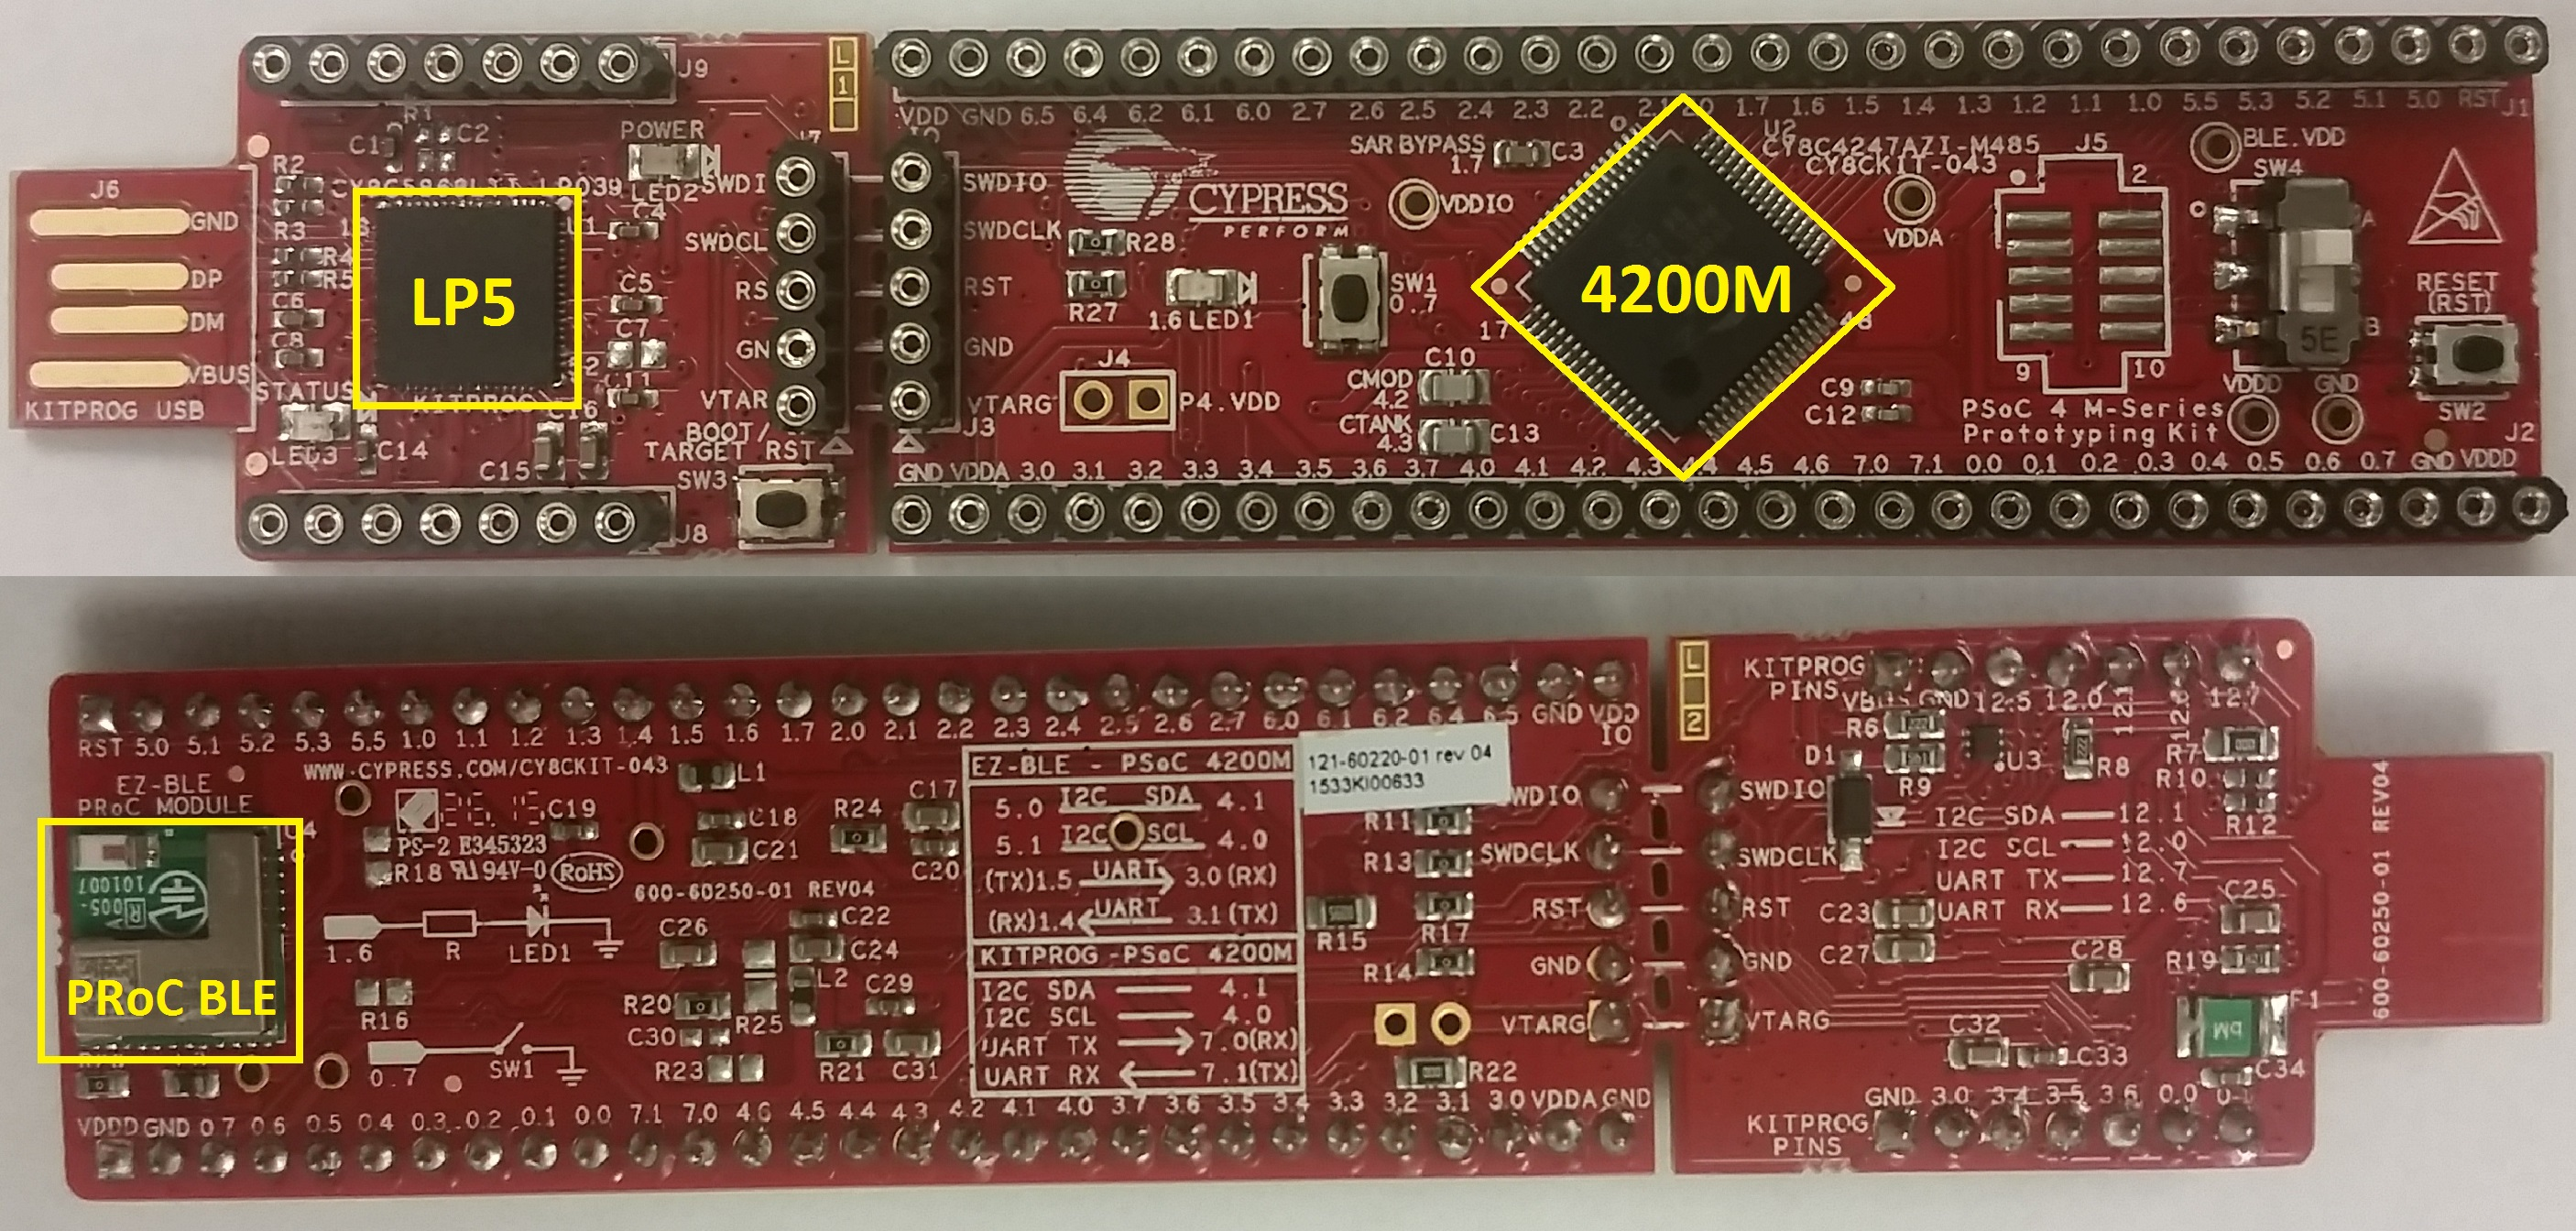
\includegraphics[scale=0.15]{figures/bProblemloesning/PSoC3.jpg}
	\caption{På figuren ses MCUen CY8CKIT-043 PSoC 4 M-Series Prototyping Kit foran og bagpå. På forsiden findes to PSoC og på bagsiden findes PRoC, som alle er tydeliggjort med gul markering og navngivning. Mikrokontrolleren kan knækkes over i to: KipProg board med USB stik og target board med hovedchippen PSoC 4200M\fxnote{Navnene er fundet nederst på side 26 i manualen}. PRoC'en er ikke påmonteret som standart fra Cypress, hvorfor denne er blevet loddet manuelt på efterfølgende. Kontakten helt til højre på forsiden af target boardet, som også er loddet manuelt på efterfølgende, skal trykkes ned for, at PRoC programmeres på istedet for PSoC 4200M. \citep{CYPRESS2016PSoC,Semiconductor2016}}
	\label{fig:PSoC}
\end{figure}\vspace{-0.2cm}
Når data skal opsamles, skal to CY8CKIT-043 PSoC 4 M-Series Prototyping Kit benyttes. Én skal placeres på personen og opsamle data, som skal sendes til en anden MCU, der er koblet til en computer via USB. Dette kan lade sig gøre, da MCUen har Inter-Integrated Circuit (I$^{2}$C) interface. I$^{2}$C er en computerbus dataprotokol, hvilket gør det muligt for de to MCUer at opføre sig som master eller slave. Rollen i kredsen bestemmes igennem softwaren. Masteren kontrollerer I$^{2}$C bussen og sender kommandoer til slaven. Både master og slave kan sende og modtage data, men masteren kontrollerer, hvornår dette kan finde sted. Det er muligt med I$^{2}$C interface at lave flere slaver eller flere masters til slaverne. I dette tilfælde vil der være én slave og én master. Disse kan kommunikere ved hjælp af et virtuelt kabel, som skabes af BLE. \citep{Semiconductor2016,Sparkfun2016}\\
Mellem PSoC LP5 og PSoC 4200M samt mellem PSoC 4200M og PRoC findes blandt andet nogle serielle porte med to ledninger til at modtage data (RX) og sende data (TX). Disse tre mikroprocessorer kommunikerer altså ikke på samme måde, som to MCUer kommunikerer med hinanden. \citep{Semiconductor2016} \\
Mikrokontrolleren kræver en ekstern strømkilde for at kunne fungere. Igennem USB porten adapteres tilslutningen til 5V, men det er muligt at tilkoble en strømkilde til boardets lav-volt applikation, hvilket gør den trådløs. 3,3V til 5,5V tilsluttes VDD fra en reguleret forsyning, hvilket er yderst essentielt, da boardet ikke besidder en elektrostatisk afladnings beskyttelse (ESD). Hvis en ekstern strømforsyning til VDD er for ustabil eller af dårlig kvalitet, kan MCUens kredsløb blive forstyrret og vil derved ikke fungere optimalt. \citep{Semiconductor2016}

Programmet PSoC Creater kan designe hardware og software til MCUen. Herigennem bliver rekonfigurerbare analoge blokke og digital programmerbar logik kombineret\fxnote{kan den fysiske hardware opbygges digitalt}, hvorved softwaren kan tilpasses de fysiske komponenter direkte igennem kodedesign. Programmet indeholder forskellige komponenter og kodeeksempler, hvilket kan blive behjælpeligt under algoritmedesignet. \citep{Semiconductor2016} \\
Når MCUen er tilsluttet computeren og debugger igennem PSoC Creater, kan matlab fungere som et grafisk bruger interface (GUI). Dette muliggør live visualisering af den data, som eksempelvis en master MCU modtager fra en slave MCU.

\subsection{Mikrokontrollerens target CPU}
Target CPU'en på CY8CKIT-043 PSoC 4 M-Series Prototyping Kit er 4200M, som besidder en ARM cortex-M0 processer og har produktnavnet CY8C4247AZI-M485. Denne er basseret på Instruction set architecture (ISA) kategorien Reduced Instruction Set Computer (RISC). ISA beskriver\fxnote{processor design teknikken}, hvordan processoren vil bearbejde dens instruktioner. ISA's kategorier kan blandt andet være complex instrucion set computer (CISC) eller RISC. En CISC baseret computer vil udføre opgaver med så få linjer som muligt. Processorens hardware opbygget til at forstå og udføre komplekse instruktioner, hvilket kræver flere transistorer end RISC metoden. RISC processorer benytter simple instruktioner, som kan forløbe inden for en clock cycle. Derimod kræver dette mere RAM, fordi hver opgave hentes ned, processeres over flere omgange og gemmes indtil færdiggjort. Denne metode tillader dog pipelinning, hvilket gør at flere instruktioner kan køre samtidig.\fxnote{fetch - decode - exicute. Mere laves samtidig} Sammenlignet er RISC processen hurtigere end CISC, men CISC computere kan udføre flere komplekse instruktioner på færre linjer end RISC. \citep{CYPRESS2016Cortexm0,Semiconductor20164200M,Yadav2016}\\
CPU'en i Cortex-M0 er en del af det 32-bit microcontroller unit (MCU) delsystem, som optimerer energibesparende drift ved hjælp af clock gating\fxnote{Clock gating saves power by adding more logic to a circuit to prune the clock tree. Pruning the clock disables portions of the circuitry so that the flip-flops in them do not have to switch states. Switching states consumes power. When not being switched, the switching power consumption goes to zero, and only leakage currents are incurred}. %% Noget om deep sleep / low power mode (Hvis den har det), hvor mange registre den har og hvis nogen af dem har dedikerede funktioner
CPU'en har en flash hukommelse på 128 kB og en 16 kB RAM af types SRAM. Algoritmen og dermed programmet for MCUen gemmes i flash, da RAM hukommelsen kræver konstant strøm og slettes dermed, hvis strømtilførslen til MCUen slukkes. \citep{Semiconductor20164200M}
%tilgængelige pins - tilkobling af perifære moduler, som f.eks. en sensor
%
\subsection{ADC}
En analog-til-digital konverter benyttes, når et analog signal skal konverteres til digital data, som kan bearbejdes eller visualiseres af en computer. Samplingsfrekvensen og opløsningen for ADCen er afgørende for, hvor korrekt det analoge signal bliver præsenteret. Ifølge Nyquist teorien skal samplingsfrekvensen være mindst det dobbelte af den højeste frekvens i signalet for, at signalet optages præsentabelt nok. Der findes flere forskellige typer ADC, som for eksempel digital ramp ADC, sigma delta ADC og successive approximation (SAR) ADC. Forskellen herimellem er metoden for konverteringen. \citep{Moore2004,Sheingold2014}

I mikrokontrolleren findes en 12 bits 1 mega sample pr sekund (Msps) SAR ADC. I en SAR ADC kommer signalet ind i en komparator, der har en spændingsværdi og sammenligne med (Vref). Først sammenlignes inputsignalet med Vref/2, og komparatoren vil vurdere, om signalet er større eller mindre end denne værdi. Herved findes det mest betydende tal først, hvorefter processen med halvering af Vref og vurdering herudfra fortsætter indtil de 12 bits er fundet. Derved er den analoge data konverteret til binære tal. Hvis en SAR ADC har for mange bits, bliver disse inddelingstrin så små, at det kan være støj, som afgør bits trinet.\fxnote{Kilden er Johns forelæsning 9, men han har ikke lagt litteratur ind, og dette er nærmest bare mine (Cecilie) noter ud fra forelæsnignen..}\\
Mikrokontrollerens 12 bits ADC kan inddele det analoge signal i $2^{12} = 4096$ spændingsniveauer og skal bruge 18 clocks for at fuldføre en 12 bits konvertering af data med samplingsfrekvens på 18.000.000 Hz, hvilket er dens maksimale samplingsfrekvens. Den understøtter både single ended og differential inputs og kan skanne alle 16 kanaler automatisk. \citep{Semiconductor20164200M,Moore2004} \\
ADCen fungerer ikke under deep sleep mode. \citep{Semiconductor20164200M}

\subsection{Interrupts}
Interrupt er en funktion, som kan afbryde CPU'ens main fil ved at løfte et ben højt, hvis en bestemt hændelse sker eller en timer har talt op til et bestemt niveau. Dette kan være behjælpeligt for CPU'en, da den herved ikke skal tjekke konstant for, om en bestemt hændelse sker. \citep{Badiger2016} \\
En PSoC 4 besidder 32 interrupt linjer, IRQ[0] til IRQ[31], som kan prioriteres efter fire niveauer. Derudover findes en wakeup interrupt controller (WIC), som vækker processoren op fra deep slepp mode. Når et interrupt finder sted, vil CPU'en modtage en specifik funktion, som kaldes Interrupt Service Routine (ISR). Denne skal sørge for, at interruptets kode overståes hurtigst muligt, hvorved mainprogrammet ikke afbrydes konstant. Interruptets kode bliver eksekveret, hvorefter main filen fortsættes. \citep{Badiger2016}\\
Inden et interrupt er mainen i tread mode, hvilket ses på \figref{fig:interrupt}. Når interruptet finder sted, vil en pind gå høj, og processoren vil overføre information til den nuværende stack. Dette kaldes for stacking, hvilket får main filen til at gå i handler mode. Her pauses den pågældende funktion, så der er mulighed for at vende tilbage til præcis samme sted i processen efter interruptet. ISR kører sit program, hvorefter pinden lægges ned igen og unstacking foregår. Main filen går igen i tread mode og fortsætter arbejdet. \citep{Badiger2016,Tanenbaum2006}
\begin{figure}[H]
	\centering
	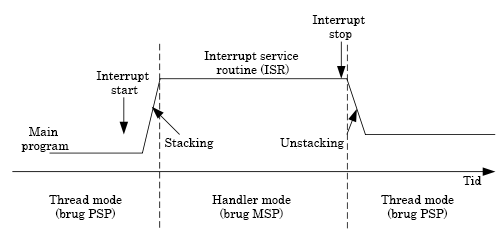
\includegraphics[scale=0.68]{figures/bProblemloesning/interrupt.png}
	\caption{På figuren ses et overblik over, hvad der sker når et interrupt afbryder CPU'ens main. \citep{Tanenbaum2006}}
	\label{fig:interrupt}
\end{figure}\vspace{-0.5cm}
I en ARM Cortex-M0 kan en høj prioritet afbryde en lav prioritet. Hver gang et interrupt finder sted, er der risiko for et stack overflow. Dette hænder, hvis afbrydelserne fortsætter i uendelighed, og det ikke er muligt af finde ud af, hvor i prosessen interruptet skal vende tilbage til. Hver gang der sker et interrupt skal otte 32-bits word på stacken. Igennem unstacking genskabes de registre fra, hvor afbrydelsen oprindeligt fandt sted.\\
Der findes to typer kilder til PSoC 4 interrupts: Fixed-function interrupt sources eller Universal Digital Block (UDB). Fixed-function interrupts er definerede interruptskilder fra on-chip perifert udstyr, som kan udløse manuelt. Herimod kan ethvert digitalt signal, som er genereret i en UDB, udløse et interrupt. Disse to typer er begge programmerbare eksterne interrupts, som i ARM Cortex M0 mikroprocessoren har lavest prioritet. Der findes fem yderligere interrupts, som kaldes exeptions og er prioriteret højere end de programmerbare eksterne interrupts. Disse eksisterer for blandt andet at genstarte processoren i tilfælde af softwarefejl\fxnote{Watch Dog timeren genstarter og har aller højest prioritet af alle interrupts}. \citep{Badiger2016}

\subsection{Clocks}
Clocks er et kredsløb, som benyttes til at synkronisere for eksempel rækkefølgen af funktioner eller indstilling af to signaler. Det kan siges, at en clock kontrollerer tiden for et program. En clock udsender en række impulser, der skifter mellem værdierne 0 og 1, med præcis pulsbredde og interval mellem hinanden. Tidsintervallet imellem to impulsers stigning til 1 eller fald fra 1 kaldes clock cycle time, og pulsfrekvensen indstilles herefter. Pulsfrekvensen styres ofte kontrolleret af en crystal oscillator, da dette gør frekvensen mere præcis. \citep{Tanenbaum2006}

Clock systemet for PSoC 4200M består af en Watch Crystal Oscillator (WCO), der kører med 32 kHz. Derudover findes en internal main oscillator (IMO), som kører med 24 MHz men kan fungere fra 3 til 48 MHz, og en internal low-speed oscillator (ILO), der nominalt kører med 32 KHz. IMO er den primære kilde til intern clocking indeni PSoC 4200M i aktiv tilstand, hvorimod ILO kan generere clocks under deep sleep mode. WCO kan både benyttes under aktiv og deep sleep mode. Denne oscillator kan desuden benyttes som en real-time clock, hvilket holder styr på den aktuelle tid.\fxnote{Når vi ved, om vi skal bruge clocks, og i så fald hvilke, kan disse eventuelt blive beskrevet her.} \citep{Semiconductor20164200M}
%http://www.hardwaresecrets.com/how-a-cpu-works/2/

\subsection{Trådløs kommunikation - BLE} 
Bluetooth er fordelagtigt at benytte, hvis der ønskes trådlås kommunikation eller trådløse enheder. PRoC'ens CPU på CY8CKIT-043 PSoC 4 M-Series Prototyping Kit er EZ\_BLE PRoC Module, som besidder en ARM cortex-M0 processer og har produktnavnet CYBLE-022001-00. Denne CPU har en 2,4 GHz BLE radio, som understøtter en datahastighed på 1 Mbps, med en chip antenne, der kan transmittere data ved radiofrekvens mellem 2400-2500 MHz. %Rundt om antennen, som sender og modtager data, er der fri plads, fordi den larmer meget og vil dermed ødelægge radioens funktion samt data.
\citep{Semiconductor2016PRoC,Semiconductor2016BLEdyb}\\
Bluetooth er en radiobølge teknologi, som hovedsageligt er designet til trådløs kommunikation imellem enheder. Der findes Bluetooth Smart enheder, som kun understøtter BLE, og Bluetooth Smart Ready enheder, der understøtter både klassisk Bluetooth og BLE. Radiobølgerne bliver sendt og modtaget i bånd af 79 forskellige frekvenser, som kandes kanaler og er centreret om 2,4 GHz, og bliver modificeret af enheden, således radiobølgerne opfattes som et signal. Når to enheder forbindes med hinanden, danner de et netværk kaldet en piconet. Enheden, som skaber forbindelsen, vil automatisk være masteren og kan for eksempel kontrollere afsendelsen af data fra slaven samt styre varigheden af forbindelsen. Tilsammen vælger masteren og slaven en tilfældig kanal, men for at mindske risikoen for interferens fra andre enheder skifter de to kanal op til tusinde gange i sekundet. \citep{CYPRESS2016workshopBLE,Sauter2011} \\
BLE er en videreudvikling og kaldes også Bluetooth version 4.0. BLE kræver mindre strøm for at fungere, fordi enheden er slukket / i sove mode størstedelen af tiden. Når data skal sendes, vil den aktivere og overføre så hurtigt som muligt for igen at deaktivere. Dette opnås ved, at BLE kun benytter 40 forskellige kanaler, hvor nogle for eksempel er specielt dedikeret til at skabe forbindelse\fxnote{3 kanaler - alm bluetooth gar 32} mellem enheder og andre til at sende data. Derved sikres en driftscyklus\fxnote{ratio mellem enheden er slukket og tændt} som er tæt på nul. Et BLE modul kan dog ikke skifte undervejs mellem master og slave rollen, hvilket betyder, at når en forbindelse er skabt, vil der være en fast master og en fast slave. Dette simplificerer designet yderligere, hvorved der ligeledes spares strøm. \citep{Gupta2013}

\subsection{UART kommunikation} %(Aktivitetsmåler til monitorering)
% RX TX
%
%
%
% I pdf'en for mikrokontrolleren - se side 23
% Skrive om I2C
%
%Denne prototyping Kit platform er ved hjælp af en computer med aktiv bluetooth i stand til at sende og modtage trådløs data fra Y8CKIT-042-BLE Bluetooth® Low Energy (BLE) Pioneer Kit platformen, som indeholder en PRoC.
%CYPRESS2016BLE
%CYPRESS2016PSoC
%Semiconductor2016
%Semiconductor2016BLE